% !TeX spellcheck = en_US
\documentclass[
    10pt,
    A4,
    english,
    draft = false,
    twoside = false,
]{article}

\usepackage{curriculum-vitae}
\usepackage{tikz}
\usepackage{graphicx}
\usetikzlibrary{calc}
\usepackage{fancyhdr}

\cfoot{\tiny{© I agree to the processing of personal data provided in this document for realising the recruitment process pursuant to the Personal Data Protection Act of 10 May 2018 (Journal of Laws 2018, item 1000) and in agreement with Regulation (EU) 2016/679 of the European Parliament and of the Council of 27 April 2016 on the protection of natural persons with regard to the processing of personal data and on the free movement of such data, and repealing Directive 95/46/EC (General Data Protection Regulation).)}}
\begin{document}
	%	Basic information	
	\setname{Piotr}{Kornaszewski}
	\setaddress{Siadło Górne 8 / 72-001 Kołbaskowo}
	\setmobile{(+48) 500 793 323}
	\setmail{kornaszewski.piotr@wp.pl}
    \setgithub{\href{https://github.com/Kanekiop1}{ Github}}
    \setlinkedin{\href{https://www.linkedin.com/in/piotr-kornaszewski-783420158/}{Linkedin}}

	%---------------------------------------------------------------------------------------
	%	Title + Contact
	%----------------------------------------------------------------------------------------
	\cvtitle{Curriculum Vitae}
	
	\begin{tikzpicture}[remember picture,overlay]
    \node[anchor=south west,inner sep=0pt, scale=0.14] at ($(current page.south west)+(15.65cm,23.4cm)$) {
     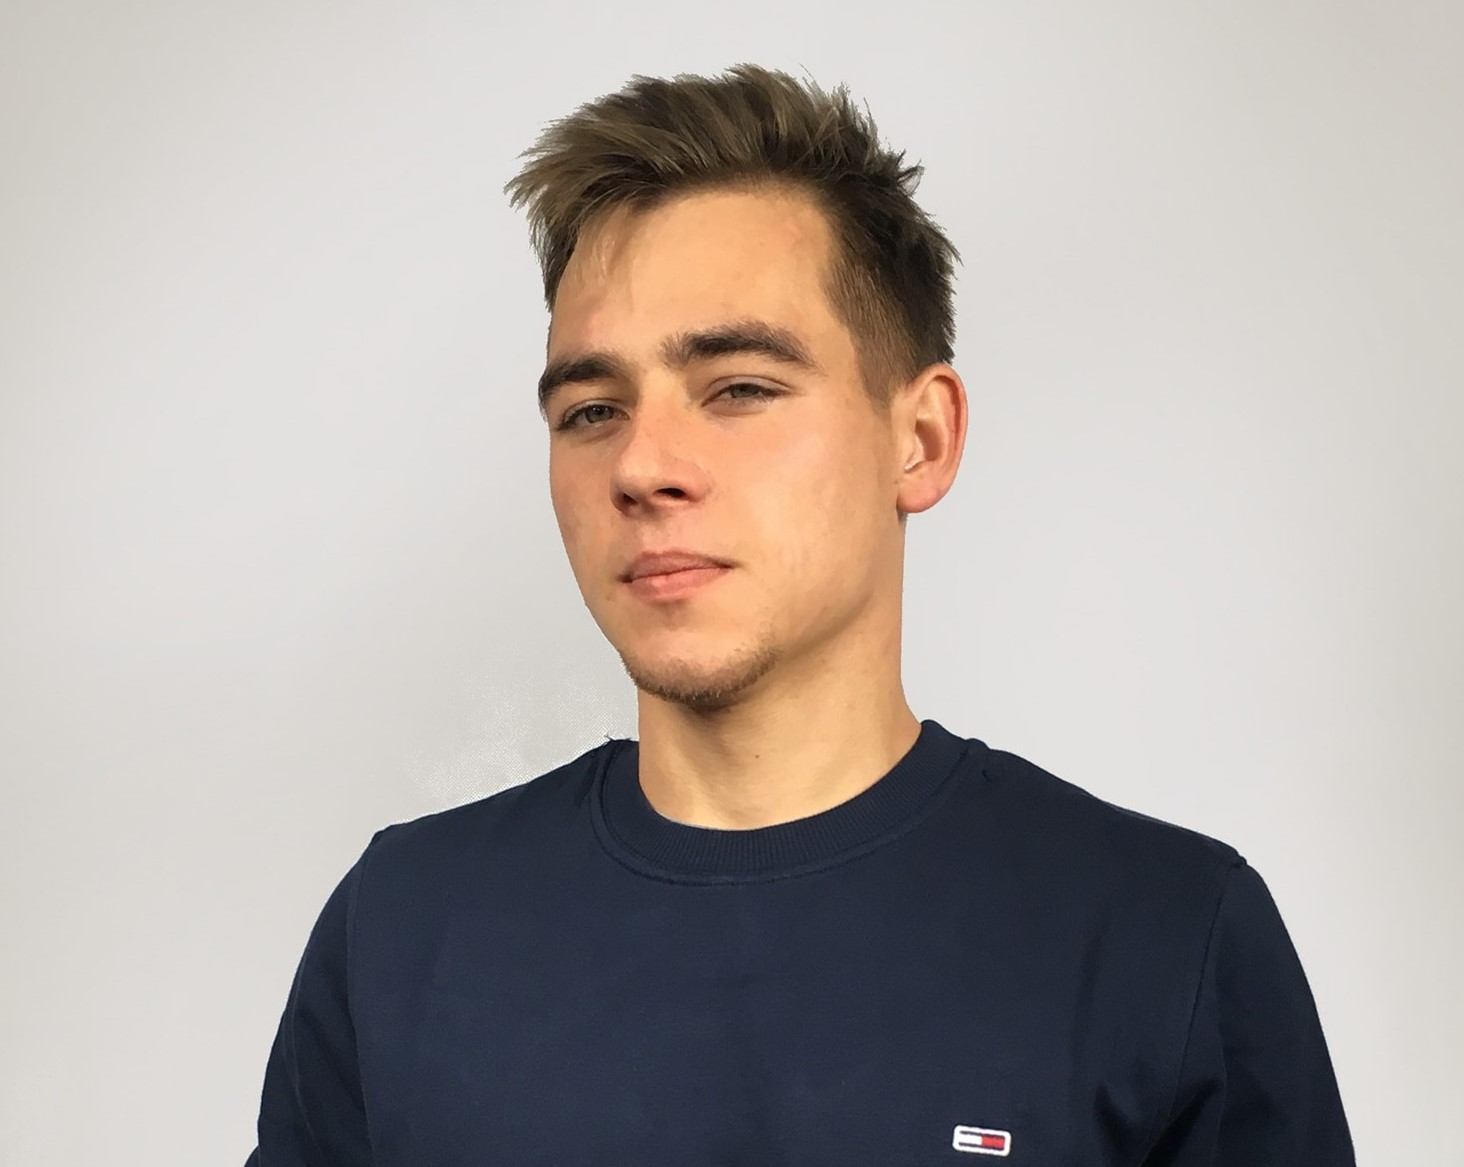
\includegraphics{cv.jpg}
     };
    \end{tikzpicture}
	\hspace{8pt}
	%---------------------------------------------------------------------------------------
	%	Summary / Objectives
	%----------------------------------------------------------------------------------------
    \cvSection{About myself}	
    \CVTextBlock{Self-motivated automation and robotics engineer equipped with close to three and a half years of experience with hardware and software. From the outset in avionic UTM and UAV field, especially drones. Always looking for new challenges and expand a knowledge.}
	%---------------------------------------------------------------------------------------
	%	Current Position
	%----------------------------------------------------------------------------------------
%	\cvSection{Current Position}
	%---------------------------------------------------------------------------------------
	%	Education
	%----------------------------------------------------------------------------------------
	
	\cvSection{Education}
	\CVBlockWithTime{West Pomeranian University of Technology in Szczecin}{2/2020 - 9/2021}
	{Electrical Department}{Szczecin, Poland}
	{\textbf{Major} Automation \& Robotics, Master's Degree Studies}
    \CVBlockWithTime{West Pomeranian University of Technology in Szczecin}{9/2016 - 2/2020}
	{Electrical Department}{Szczecin, Poland}
	{\textbf{Major} Automation \& Robotics, Master's Enginer Studies}
	%---------------------------------------------------------------------------------------
	%	Experience (Research and Industry)
	%----------------------------------------------------------------------------------------
%	\cvSection{Experience (Research \& Industry)}
	\cvSection{Expierience}
	\CVBlockWithTime{Hardware and software tester}{1/2022 - current}{Aerobits Sp. z o.o.}{Szczecin, Poland}
	{Writing hardware tests using Python, Linux/Bash language, validating software and preparing technical documentation}	
    \CVBlockWithTime{Electronics Engineer}{8/2021 - 12/2021}{Aerobits Sp. z o.o.}{Szczecin, Poland}
	{Assembly of prototype radio modules, fault diagnosis and preparation of technical documentation} 
    \CVBlockWithTime{Electronics Technician}{7/2019 - 8/2021}{Aerobits Sp. z o.o.}{Szczecin, Poland}
	{Assembly, repair of radio modules and preparation of technical documentation}

	%---------------------------------------------------------------------------------------
	%	Skills
	%----------------------------------------------------------------------------------------
	\cvSection{Skills}
	\tab \begin{tabular}{r p{0.7\textwidth}}
		\texttt{\large Programming languages} & \textbf{Python} 
		   - writing hardware test blocks using UART/USB communication and software tests,
            database applications (DB, SQLite), 
            extracting tables from web pages and data processing, \newline 
        \textbf{GitHub} - creation and maintenance of CI according to project guidelines, \newline
        \textbf{Latex} - preparation of technical documentation, as well as sales documentation, \newline
        \textbf{Matlab} - use of global optimization toolbox to generate mobile robot trajectories, \newline
        \textbf{C} - remote controller app using Arduino and nRF24 module, \newline
        \textbf{C\#} - object-oriented application to operate an industrial manipulator using RS232 transmission, \newline
        \textbf{Linux\textbackslash Bash} - simple system scripts using Python application functionalities \\
		\texttt{\large Environments \& Tools} & Git \cvContactSep Windows \cvContactSep Linux \cvContactSep Matlab \cvContactSep Jupyter \cvContactSep VSCode \cvContactSep Texstudio \\
		\texttt{\large Languages} & \textbf{Native:} Polish \cvContactSep \textbf{Other:} English (B1/B2)  \\
        \texttt{\large Soft} & Hardworking \cvContactSep Conscientiousness \cvContactSep Teamwork   \\
	\end{tabular}\\~\\
	
	%----------------------------------------------------------------------------------------
\end{document}